\begin{frame}
  \frametitle{MatLabb}
  \framesubtitle{Klasser och datatyper}
  \begin{itemize}
  \item \textbf{Klasser}
    \begin{itemize}
    \item \texttt{Shell, Recipe, Lookup, (SearchTerm)}
    \item \texttt{InfoIngredient, RecipeIngredient, (Ingredient)}
    \end{itemize}
  \item \textbf{Structs}
    \begin{itemize}
    \item \texttt{MiniRecipe, RelatedRecipe}
    \end{itemize}
  \end{itemize}
\end{frame}

\begin{frame}[c]
  \frametitle{MatLabb}
  \framesubtitle{Klassdiagram}
  \centering
  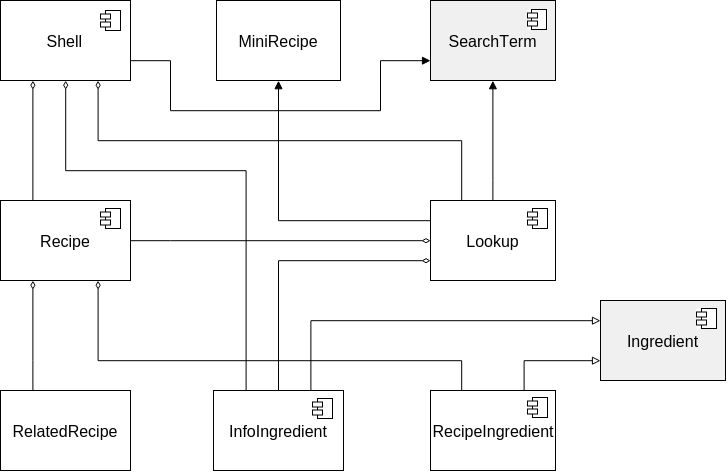
\includegraphics[scale=.36]{klass-bantad.png}
\end{frame}
